\documentclass[12pt]{article}
\usepackage[pdftex]{graphicx}
\usepackage{hyperref}

\setlength{\oddsidemargin}{1.4cm}
\setlength{\evensidemargin}{0.1cm} 
\begin{document}

%---------------------------Titelseite-----------------------------------------
\title{ \bf \LARGE Ebbe und Flut 1.0.2}

\author{Wolfgang Werner - Idea\\
        Peter Karich - Programmer\\ }
\maketitle
%------------------------------------------------------------------------------


%------------------------------------INHALT-------------------------
\setcounter{tocdepth}{2}
\tableofcontents

\newpage
%------------------------------------------------------------------------------
\pagestyle{headings}

\section{Introduction}
The Idea is from Wolfgang Werner. The publisher  -Adlung- offers Ebbe und Flut 
(this means low tide and high tide) as cardgame for 7 EUR.\\
I want that others understand this program as substitution for the one player modus, because in
the card game this modus makes not really fun.\\
We can find out, wether player one or two will win the game if there are the same (best) players.
A good training is, to look how the pc's play against each other.
\section{Installation}
You'll need a java virtual machine (jvm)! On common systems this is preinstalled. The minimum is version 1.1.
The newest and old versions are available on http://java.sun.com . But this versions are over 10 MB big. 
So support open source engine on www.kaffe.org.
\subsection{Linux}
Copy all files in your favourite directory, than go there with the terminal and type in {\bf ./linuxStart.sh}!
\subsection{Windows}
Copy all files in your favourite directory. Than click on winStart(.bat).
\subsection{Mac}
The same procedure as discribed under Linux.
\subsection{Zaurus}
Either use the ipk file under zaurus/ or create the ipk file with the provided script.
See also this
\href{http://www.oesf.org/index.php?title=IPKG_Howto}{how to}.
\section{Laws}
\subsection{Overview how a move looks like}
\subsubsection{Check}
\label{ueberpruefen}
This Step is not a must!
If your oppponent forgot some moves (he could move cards), you can click on his finishstack and so 
he will never do it again, because now he lose a finished card!\\
So you should be sure for your self, that you have done all moves!\\
After that your opponent has to move all his possible cards, if he don't want to lose another finished card.\\
May be your opponent hasn't forgot any move, or it's your first one than skip this step!
\subsubsection{Uncover The Card}
This Step is a must!
Click on the startstack. Now you should see the next card, you can place this card on one of your
startfields.
Sometimes you can move cards before this placing, if you want to do that. This can be the case, if the 
moves of your opponent uncover some cards.\\
If you click on the startstack and nothing happens, may be you forgot some move and so your opponent
can do step: check \ref{ueberpruefen}. Now you have to do all possible moves.
or may be there are no cards! Now we are close to the end. See Chapter \ref{ende}.
\subsubsection{Place Uncovered Card}
This step is a must!
You move the card from startstack to one of your startfields: : 44, 34 und 43 for player one and 
00, 01 und 10 for player 2.\\
In the program click on the startstack and than on one of the three fields.
\subsubsection{Move Cards}
This step is not a must.
Move until no move is possible :-).
The moving for player one (for player two rotate your board with $180 \circ$ ):\\
If a value or a character from one of your cards, is equal to the value or the character from another of your
cards in the horizontal line, than you can move one of the cards one field up.\\
If a value or a character from one of your cards, is equal to the value or the character from another of your
cards in the vertical line, than you can move one of the cards one field to the left.\\
If one of these both cases happens, i will call it "same" cards.
You move a card in the game, if you click the card and than the field where you want to place it again.
\subsubsection{End Your Move}
This step is a must!
Be sure you are ready (no own moves possible), before you end your move!
Click the startstack! Now your opponents move follow.
\subsection{Important Things}
\subsubsection{}
Sometimes it is the case that you could move one card out of the board. (two same cards on the upper or left edge for player one => Now you could move one of these out of the 5x5 board). In the program it is a little bit complicated. Go to "`Card"' in the menu and click "`remove"'. Now you will see: "`Click the card you want to move out of board!"'. Press Ok and than click the card you want to move out of the board. You will get a message if it is not possible.\\
This step makes sense, because if you don't do this your opponent could make step: check \ref{ueberpruefen}. In most cases you can prevent these situations!
\subsubsection{}
If you move cards you could covered others. In the program you can look how much cards are on a field and color they have. Click on "`Card"' in the menu and than "`show Stack"'. Now you will see: "`Click the stack you want to see!"'. Click Ok, and than the field. Now a window with some cards will pop up. Only the first card is visible the other will replaced by a -?- character.
\subsection{End}
\label{ende}If both players can't move anything and their startstacks are empty, than the game is finished! \subsection{Gamegoal}
The one who has the most finished cards (cards in the finishstack), is the winner. If you go with your own card on the oppponents startfields, this card will moved to your finishstack indeed. In the program it will happens automatically.
\subsection{Example}
At the beginning each player has 25 cards on his startstack:\\ A1, A2, A3,A4, A5, B1, ..., E5 
for player one and a1, ..., e5 for player two\\ This stacks are mixed and covered. Player one starts(always). He is the player on the down side. He uncoveres his first card (he clicks on his startstack and see e.g. B5) and than he places this card to his startfields 44, 34 und 43. (click on startstack and than e.g he clicks on 44) Now he is ready, so he clicks startstack again to end his move. Player two places a1 on the field 00.\\
Now again player one is on turn: he uncoveres E5 and places it to 43. Now he can move E5 or B5 one field to the left.(Click on e.g. card E5, which will lightup in red color and than click field 33)
\newpage
\subsection{Overview}
All visible fields are in the reallifecardgame cardSTACKS. So the fields could be empty or filled with up to 25 
cards or even more.
I call the numbered fields 00 until 44 as gameboard(5x5).\\
fields 44, 34 and 43 = startfields of player one= finishfields of player two\\
fields 00, 10 and 01 = startfields of player two= finishfields of player one\\
at the beginning startstacks 1 and 2 contain 25 cards.\\
at the beginning finishstacks one and two are empty.\\
"`turn No.?"' shows which move number is the actual one.
\begin{figure}[ht]
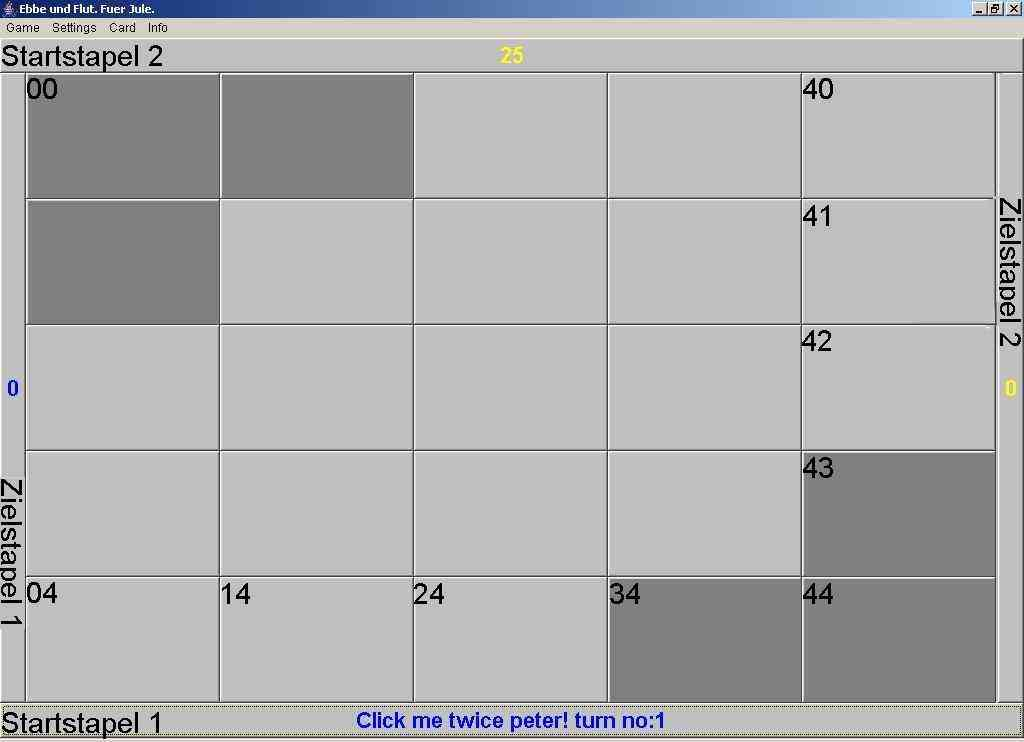
\includegraphics[scale=0.5]{overview.jpg}
\label{overview}
\caption{startconstellation}
\end{figure}
\section{Outro}
Now have fun!\\
Please report bugs to {\bf sourcemaker2000-berlios@yahoo.de}. And visit {\bf http:/developer.berlios.de/ebbeflut} for the newest version.\\
I hope you understand my English! Please send me better translations of liesmich.tex :-)!
\section{License}
Copyleft Peter Karich 2004. This program stands under the GPL(general public license)! 
There is no WARRANTY for the functionality of the program!
 "`If the software is modified by someone else and passed on, we want its
recipients to know that what they have is not the original, so that any problems
introduced by others will not reflect on the original authors' reputations."')
Read gpl.txt for more information or visit www.gnu.org!
\end{document}
